\documentclass[aspectratio=169,10pt]{beamer}

% Theme & Styling
\usetheme{Boadilla}
\usecolortheme{whale}

% Typography & Color definitions
\usepackage[T1]{fontenc}
\usepackage{lmodern}
\usepackage{tikz}
\usetikzlibrary{shapes.geometric, arrows.meta, positioning, calc}
\usepackage{booktabs}
\usepackage{tabularx}
\usepackage{colortbl}
\usepackage{amsmath}

% Custom Palette
\definecolor{NavyBlue}{RGB}{16, 44, 87}
\definecolor{SlateCyan}{RGB}{53, 162, 159}
\definecolor{SoftGray}{RGB}{245, 247, 250}
\definecolor{AccentGreen}{RGB}{34, 139, 34}
\definecolor{AccentRed}{RGB}{178, 34, 34}
\definecolor{DarkText}{RGB}{30, 30, 30}

\setbeamercolor{palette primary}{bg=NavyBlue,fg=white}
\setbeamercolor{palette secondary}{bg=SlateCyan,fg=white}
\setbeamercolor{palette tertiary}{bg=NavyBlue!80,fg=white}
\setbeamercolor{structure}{fg=NavyBlue}
\setbeamercolor{title}{fg=NavyBlue}
\setbeamercolor{frametitle}{bg=NavyBlue,fg=white}
\setbeamercolor{block title}{bg=NavyBlue,fg=white}
\setbeamercolor{block body}{bg=SoftGray,fg=DarkText}

\setbeamertemplate{navigation symbols}{}
\setbeamertemplate{footline}[frame number]

% Metadata
\title[\textbf{Project Hephaestus} | AMD Kria KR260]{\textbf{Project Hephaestus: Edge-Accelerated Neural Policy \& Hardware Safety Gate}}
\subtitle{Turnkey Heterogeneous PS-PL Co-Design for AMD Kria KR260 Robotics Starter Kit}
\author[\textbf{Brian A. Hadian}]{\textbf{Brian A. Hadian}}
\institute[AMD Kria KR260 Robotics]{Autonomous Robotics \& Hardware Acceleration \\ AMD Zynq UltraScale+ MPSoC (xck26-sfvc784-2LV-c)}
\date{\today}

\begin{document}

% ==============================================================================
% SLIDE 1: Title & Overview (Single Insight: Offloading to PL delivers safety & efficiency)
% ==============================================================================
\begin{frame}
    \titlepage
    \vspace{-1.2em}
    \begin{block}{\centering \textbf{Core System Insight}}
        \centering
        \small
        Offloading neural obstacle avoidance policies to AMD Kria KR260 FPGA Programmable Logic guarantees \textbf{deterministic sub-millisecond execution ($138.3\,\mu\text{s}$)}, \textbf{zero-latency hardware fail-closed safety}, and \textbf{$271\times$ higher energy efficiency} compared to traditional host CPU control loops.
    \end{block}
\end{frame}

% ==============================================================================
% SLIDE 2: Heterogeneous Hardware Architecture (Single Insight: PS handles perception, PL handles real-time compute & safety)
% ==============================================================================
\begin{frame}{Heterogeneous System Architecture: PS-PL Partitioning}
    \begin{block}{\textbf{Key Architectural Insight}}
        High-level robotics perception and networking run on the Linux Processing System (PS), while neural policy evaluation and safety gates execute deterministically at wire-speed on the UltraScale+ Programmable Logic (PL).
    \end{block}
    
    \vspace{0.1em}
    \begin{columns}[T]
        \begin{column}{0.49\textwidth}
            \begin{block}{\textbf{Processing System (PS) — ARM Cortex-A53}}
                \begin{itemize}\footnotesize\setlength{\itemsep}{1pt}
                    \item \textbf{Operating System:} Ubuntu 22.04 LTS (64-bit ARMv8).
                    \item \textbf{Direct Bus Access:} Pure Python \texttt{/dev/mem} driver via high-speed memory-mapping (Zero C++ dependency).
                    \item \textbf{On-Target Management:} Linux FPGA Manager (\texttt{xmutil} \& \texttt{/sys/class/fpga\_manager}) for dynamic bitstream loading without reboot.
                \end{itemize}
            \end{block}
        \end{column}
        
        \begin{column}{0.49\textwidth}
            \begin{block}{\textbf{Programmable Logic (PL) — UltraScale+ MPSoC}}
                \begin{itemize}\footnotesize\setlength{\itemsep}{1pt}
                    \item \textbf{Neural Accelerator:} 8-lane parallel MAC core ($74 \rightarrow 128 \rightarrow 64 \rightarrow 3$ MLP) mapped to 16 DSP48E2 slices and 8 Block RAM banks.
                    \item \textbf{Deterministic Core Latency:} Exactly \textbf{6,916 clock cycles} ($138.32\,\mu\text{s}$ @ 50\,MHz) with 40-bit non-overflow accumulators.
                    \item \textbf{Hardware Safety Gate:} Autonomous monotonic 20\,ms lease watchdog, physical/software E-Stop latch, and rate limiter.
                \end{itemize}
            \end{block}
        \end{column}
    \end{columns}
\end{frame}

% ==============================================================================
% SLIDE 3: Robotics Dataflow & Dual-Link Redundancy (Single Insight: Gigabit Ethernet delivers 10x lower latency with UART failover)
% ==============================================================================
\begin{frame}{End-to-End Robotics Dataflow \& Dual-Link Redundancy}
    \begin{block}{\textbf{Key Interconnect Insight}}
        A high-speed Gigabit Ethernet UDP link delivers perception data with $10\times$ lower latency than UART, backed by instantaneous, zero-latency hardware UART failover to guarantee unbroken control continuity.
    \end{block}

    \vspace{0.4em}
    \centering
    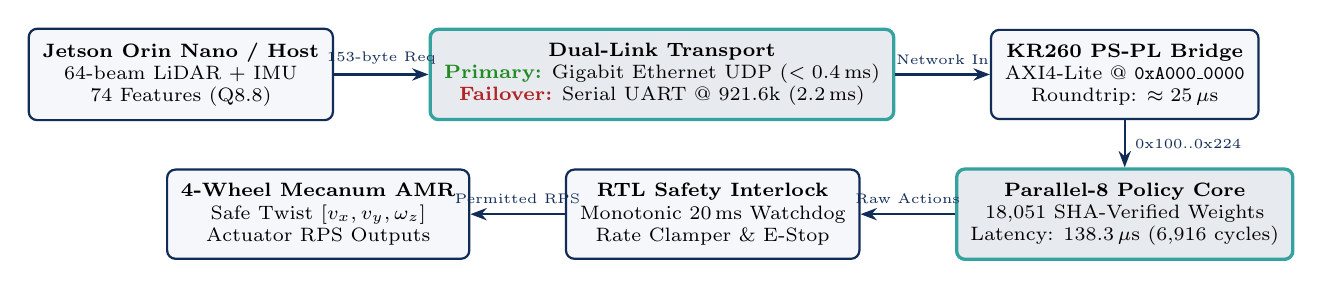
\begin{tikzpicture}[
        node distance=0.85cm,
        box/.style={draw=NavyBlue, fill=SoftGray, thick, rounded corners=3pt, align=center, font=\scriptsize, inner sep=5pt},
        hwbox/.style={draw=SlateCyan, fill=NavyBlue!10, very thick, rounded corners=3pt, align=center, font=\scriptsize, inner sep=5pt},
        arrow/.style={-{Stealth[scale=0.9]}, thick, color=NavyBlue}
    ]
        % Nodes
        \node[box] (jetson) {\textbf{Jetson Orin Nano / Host} \\ 64-beam LiDAR + IMU \\ 74 Features (Q8.8)};
        \node[hwbox, right=1.2cm of jetson] (transport) {\textbf{Dual-Link Transport} \\ \textcolor{AccentGreen}{\textbf{Primary:}} Gigabit Ethernet UDP ($<0.4\,\text{ms}$) \\ \textcolor{AccentRed}{\textbf{Failover:}} Serial UART @ 921.6k ($2.2\,\text{ms}$)};
        \node[box, right=1.2cm of transport] (axi) {\textbf{KR260 PS-PL Bridge} \\ AXI4-Lite @ \texttt{0xA000\_0000} \\ Roundtrip: $\approx 25\,\mu\text{s}$};
        \node[hwbox, below=0.6cm of axi] (plcore) {\textbf{Parallel-8 Policy Core} \\ 18,051 SHA-Verified Weights \\ Latency: $138.3\,\mu\text{s}$ (6,916 cycles)};
        \node[box, left=1.2cm of plcore] (safety) {\textbf{RTL Safety Interlock} \\ Monotonic 20\,ms Watchdog \\ Rate Clamper \& E-Stop};
        \node[box, left=1.2cm of safety] (actuation) {\textbf{4-Wheel Mecanum AMR} \\ Safe Twist $[v_x, v_y, \omega_z]$ \\ Actuator RPS Outputs};

        % Connections
        \draw[arrow] (jetson) -- node[above, font=\tiny] {153-byte Req} (transport);
        \draw[arrow] (transport) -- node[above, font=\tiny] {Network In} (axi);
        \draw[arrow] (axi) -- node[right, font=\tiny] {0x100..0x224} (plcore);
        \draw[arrow] (plcore) -- node[above, font=\tiny] {Raw Actions} (safety);
        \draw[arrow] (safety) -- node[above, font=\tiny] {Permitted RPS} (actuation);
    \end{tikzpicture}
    
    \vspace{0.4em}
    \begin{alertblock}{\small \textbf{Failover Protection Guarantee}}
        If Ethernet cable disconnects or times out ($>15\,\text{ms}$), the client \textbf{seamlessly falls back to UART} without violating the robot's $20\,\text{ms}$ deadline.
    \end{alertblock}
\end{frame}

% ==============================================================================
% SLIDE 4: Comprehensive Multi-Platform Benchmark (Single Insight: PL is 271x more energy-efficient with zero jitter)
% ==============================================================================
\begin{frame}{Multi-Platform Performance \& Power Benchmark}
    \begin{block}{\textbf{Key Benchmark Insight}}
        The AMD Kria KR260 FPGA PL achieves \textbf{$271\times$ higher energy efficiency} and \textbf{zero OS jitter} compared to host CPUs, completing full neural inference in exactly \textbf{$138.3\,\mu\text{s}$} at only \textbf{0.28\,W} dynamic power.
    \end{block}

    \vspace{0.2em}
    \centering
    \scriptsize
    \begin{tabularx}{\textwidth}{lXXX}
        \toprule
        \rowcolor{NavyBlue!15}
        \textbf{Performance Metric} & \textbf{Laptop Host CPU} & \textbf{KR260 ARM Cortex-A53} & \textbf{KR260 FPGA PL (Ours)} \\
        \midrule
        \textbf{Target Silicon} & Intel 12th Gen (x86\_64) & Quad ARM Cortex-A53 & \textbf{AMD UltraScale+ MPSoC} \\
        \textbf{Compute Clock} & $3.30 - 4.50\,\text{GHz}$ & $1.33\,\text{GHz}$ & \textbf{$50.0\,\text{MHz}$ (DSP48E2)} \\
        \textbf{Inference Latency} & $\approx 200 - 450\,\mu\text{s}$ (C/NumPy) & $\approx 450 - 1,200\,\mu\text{s}$ (NEON) & \textbf{$138.32\,\mu\text{s}$ (Exact 6,916 cycles)} \\
        \textbf{Execution Jitter} & $\pm 50 - 500\,\mu\text{s}$ (OS interrupts) & $\pm 200 - 1,500\,\mu\text{s}$ (Linux) & \textbf{$0.00\,\mu\text{s}$ (Zero Clock Jitter)} \\
        \textbf{Active Power (Core)} & $\approx 35.0\,\text{W}$ (Package TDP) & $\approx 3.78\,\text{W}$ (Measured INA260) & \textbf{$0.28\,\text{W}$ (PL Neural Dynamic)} \\
        \textbf{Energy per Inference} & $\mathbf{10,500\,\mu\text{J}}$ & $\mathbf{3,024\,\mu\text{J}}$ & $\mathbf{38.7\,\mu\text{J}}$ \\
        \rowcolor{SlateCyan!20}
        \textbf{Relative Efficiency} & $1.0\times$ (Baseline) & $3.5\times$ more efficient & \textbf{$271\times$ More Energy Efficient} \\
        \textbf{Hardware Safety Gate} & None (OS Dependent) & None (OS Dependent) & \textbf{Fail-Closed Monotonic Watchdog} \\
        \bottomrule
    \end{tabularx}
\end{frame}

% ==============================================================================
% SLIDE 5: Key Takeaways & Deployment Readiness (Single Insight: Production-ready turnkey system with automated runner)
% ==============================================================================
\begin{frame}{Key Takeaways \& Field Deployment Readiness}
    \begin{block}{\textbf{Key Deployment Insight}}
        Project Hephaestus delivers a production-ready, fully turnkey hardware accelerator for autonomous mobile robots with single-command testing, interactive diagnostics, and complete author attribution.
    \end{block}

    \vspace{0.4em}
    \begin{columns}[T]
        \begin{column}{0.48\textwidth}
            \begin{block}{\textbf{Field-Proven Capabilities}}
                \begin{itemize}\small
                    \item \textbf{100\% Bit-Exact Parity:} 16/16 golden test vectors validated against the neural policy oracle.
                    \item \textbf{Autonomous Hardware Safety:} Fail-closed 20\,ms watchdog cuts motor torque in \textbf{0\,ns} if communication halts.
                    \item \textbf{Redundant Interfaces:} High-speed AXI4-Lite ($25\,\mu\text{s}$) + Gigabit Ethernet ($<0.4\,\text{ms}$) + UART ($2.2\,\text{ms}$).
                \end{itemize}
            \end{block}
        \end{column}

        \begin{column}{0.48\textwidth}
            \begin{block}{\textbf{Turnkey Software Integration}}
                \begin{itemize}\small
                    \item \textbf{Interactive Unified Runner:} \texttt{./run\_kr260.sh} with 10 diagnostic options including live telemetry and latency benchmarks.
                    \item \textbf{Automated CI/CD Test:} \texttt{make test} and \texttt{make test-eth} execute automated headless regressions.
                    \item \textbf{Author:} \textbf{Brian A. Hadian} \\ Project Hephaestus: AMD Kria KR260 Accelerator Suite.
                \end{itemize}
            \end{block}
        \end{column}
    \end{columns}
\end{frame}

\end{document}
